%\videotitle{DARTS: Differentiable Architecture Search}


%----------------------------------------------------
\myframetop{DARTS: Differentiable Architecture Search \litw{\href{https://openreview.net/forum?id=S1eYHoC5FX}{Liu et al, 2018}}}{
	\myit{
		\footnotesize
		\item Use one-shot model with continuous architecture weight $\alpha$ for each operator
        \myit{
			\item[] $x^{(j)} = \sum_{i<j}\tilde{o}^{(i,j)}(x^{(i)}) = \sum_{i<j}\sum_{o\in\mathcal{O}}\frac{exp(\alpha_{o}^{(i,j)})}{\sum_{o^{\prime}\in\mathcal{O}}exp(\alpha_{o^{\prime}}^{(i,j)})}o(x^{(i)})$
%            \item[-] $o^{(i,j)} \in \argmax_{o\in\mathcal{O}}\alpha_{o}^{(i,j)}$
		}

		\begin{columns}
			\column{0.05\textwidth}
			\column{0.3\textwidth}
			    \centering
			    {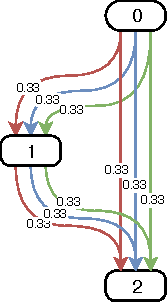
\includegraphics[scale=0.7]{images/dartsA.pdf}}\\
			    {\scriptsize (a) Initialization}
			\column{0.3\textwidth}
\onslide<2->{
			    \centering
			    {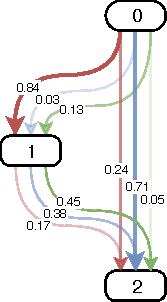
\includegraphics[scale=0.7]{images/dartsB.pdf}}\\
			    {\scriptsize (b) Search end}
}
			\column{0.3\textwidth}
\onslide<3->{
			    \centering
			    {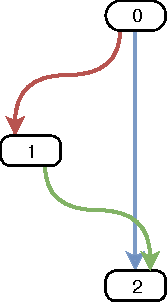
\includegraphics[scale=0.7]{images/dartsC.pdf}}\\
			    {\scriptsize (c) Final cell}
}
			\column{0.05\textwidth}
        \end{columns}
			
		\medskip
		\pause
\onslide<2->{
		\footnotesize
		\item By optimizing architecture weights $\alpha$ DARTS assigns importance to each operation.
}		
\medskip	
\pause
	
\vspace*{-0.2cm}
\onslide<3->{
	\footnotesize
	\item In the end, discretize to obtain a single architecture (c)
}
	
	}
}

%----------------------------------------------------------------------

%----------------------------------------------------

\myframe{DARTS: Architecture Optimization}{


\begin{algorithm}[H]
 %\footnotesize
 create mixed ops $\tilde{o}$ parametrized by $\alpha_{o}^{(i,j)}$ for each edge $(i,j)$\\
 \While{\textit{not converged}}{
  Update one-shot weights $\vec{w}$ by $\nabla_{\vec{w}}\mathcal{L}_{train}(\vec{w}, \vec{\alpha})$\\
  Update architectural parameters $\alpha$ by $\nabla_{\alpha}\mathcal{L}_{valid}(\vec{w}, \vec{\alpha})$\;
 }
 return $\argmax_{o\in\mathcal{O}}\alpha_{o}^{(i,j)}$ for each edge $(i,j)$\;
 \caption{DARTS 1st order}
\end{algorithm}

\centering

\myit{
	\item Solve a bi-level optimization problem (a $\rightarrow$ b) to optimize architecture $\alpha$ and weights $w$, using alternating SGD steps
}

\footnotesize{
			\begin{tcolorbox}[width = 8cm,halign=center,valign=center]
%		\begin{eqnarray}
			%\nonumber			
			$\text{min}_{\alpha} \mathcal{L}_{\text{val}}(w^*(\alpha), \alpha)$\\
			%\nonumber			
			$s.t.\ w^*(\alpha) \in \text{argmin}_{w} \mathcal{L}_{\text{train}}(w,\alpha)$
%		\end{eqnarray}
	\end{tcolorbox}
}

}
%----------------------------------------------------

%%%%%%%%%%%%%%%%%%%%%%%%%%%%%%%%%%%%%%%%%%%%%%%%%%%%%%%%%%%%%%%%%%%%%%%
\myframetop{Works quite well on many benchmarks}{

\begin{itemize}
    \item Original CNN space: 8 operations on each MixedOp
    \item 28 MixedOps in total
    \item $> 10^{23}$ possible architectures
    \item $<3\%$ on CIFAR-10 in less than 1 GPU day of search
\end{itemize}

\vspace{1cm}
\centering
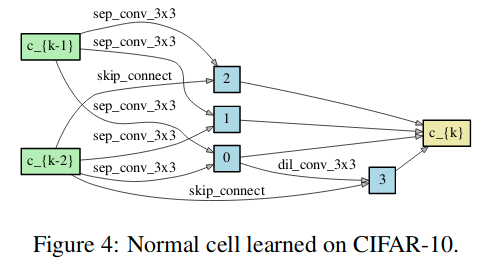
\includegraphics[scale=0.35]{images/darts_normal_cell.png}
\hspace{1cm}
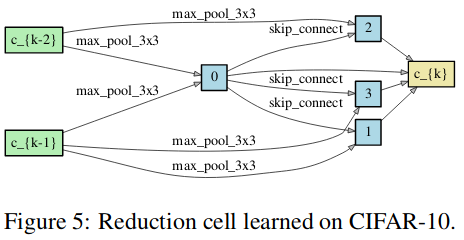
\includegraphics[scale=0.35]{images/darts_reduction_cell.png}

}
%%%%%%%%%%%%%%%%%%%%%%%%%%%%%%%%%%%%%%%%%%%%%%%%%%%%%%%%%%%%%%%%%%%%%%%%%%%%%


%%%%%%%%%%%%%%%%%%%%%%%%%%%%%%%%%%%%%%%%%%%%%%%%%%%%%%%%%%%%%%%%%%%%%%%
\myframetop{Issues -- Memory constraints}{

\small
DARTS requires keeping the whole one-shot model together with its computed tensors in memory.
    \myit{
    	\visible<2->{
    	\item[-] Constraints the search space size and the fidelity one uses to train the one-shot model.
    	}
    	\visible<3->{
    	\item[-] Not possible to run on large datasets as ImageNet.
    	}
    }

\medskip

\begin{minipage}{.45\textwidth}
\small
\visible<4->{A lot of research done to fix this issue:}

\myit{
\visible<5->{
	\item \alert{ProxylessNAS} \lit{\href{https://openreview.net/pdf?id=HylVB3AqYm}{Cai et al, 2019}} -- keeps only two edges at a time in memory
	}
\visible<6->{
	\item \alert{GDAS} \lit{\href{https://arxiv.org/pdf/1910.04465.pdf}{Dong et al, 2019}} -- by using a Gumbel Softmax it allows to keep only a single architecture in memory
	}
\visible<7->{
	\item \alert{PC-DARTS} \lit{\href{https://arxiv.org/pdf/1907.05737.pdf}{Xu et al, 2020}} -- perform the search on a subset of the total computed channels in the one-shot model
	}
}
\end{minipage}
\hspace{.5cm}
\begin{minipage}{.2\textwidth}
\visible<6->{
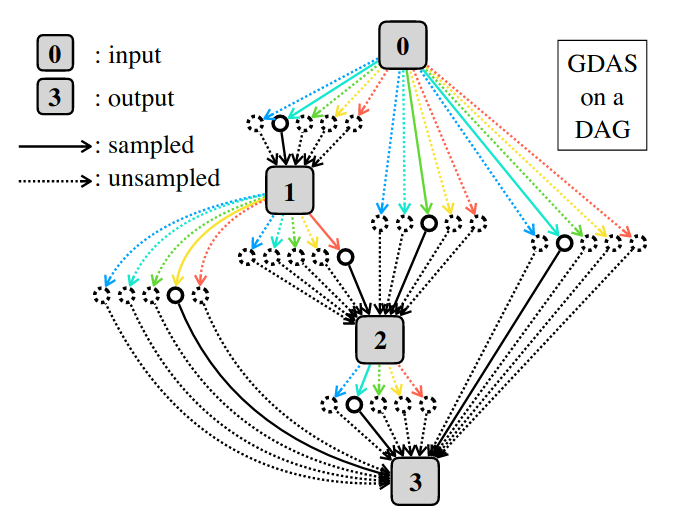
\includegraphics[scale=0.35]{images/gdas.png}
}
\end{minipage}

}
%%%%%%%%%%%%%%%%%%%%%%%%%%%%%%%%%%%%%%%%%%%%%%%%%%%%%%%%%%%%%%%%%%%%%%%%%%%%%

%%%%%%%%%%%%%%%%%%%%%%%%%%%%%%%%%%%%%%%%%%%%%%%%%%%%%%%%%%%%%%%%%%%%%%%
\myframetop{Issues -- Non-robust behaviour}{

\small
DARTS has its own hyperparameters, e.g. one-shot learning rate, $L_2$ regularization, etc.
    \myit{
    	\visible<2->{
    	\item[-] The default ones are not always optimal. Tuning these hyperparameters for every new task/search space is computationally expensive.
    	}
    	\visible<3->{
    	\item[-] DARTS may return degenerate architectures, e.g. cells composed with only skip connections
    	}
    }

\medskip

\begin{minipage}{.45\textwidth}
\small
\myit{
\visible<4->{
	\item \alert{RobustDARTS} \lit{\href{https://openreview.net/forum?id=H1gDNyrKDS}{Zela et al, 2020}} -- tracks the curvature of the validation loss and early stops the search based on that.
	}
}
\end{minipage}
\hspace{.5cm}
\begin{minipage}{.45\textwidth}
\only<3>{
	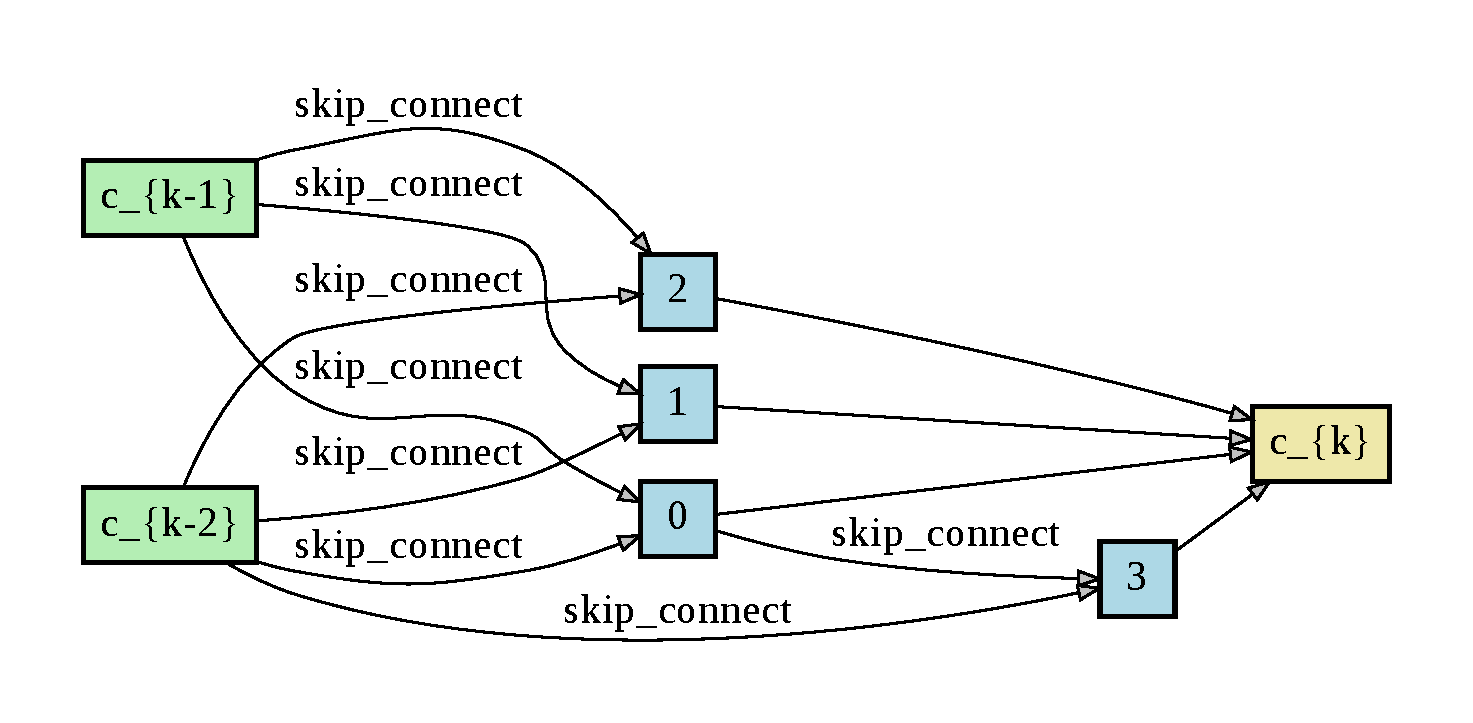
\includegraphics[scale=0.3]{images/normal_DARTS_S3.pdf}
}
\myit{
\visible<5->{
	\item \alert{SmoothDARTS} \lit{\href{https://arxiv.org/pdf/2002.05283.pdf}{Chen and Hsieh, 2020}} -- applies random perturbation and adversarial training to avoid bad regions
	}
	}
\end{minipage}

\medskip

\centering
\visible<4->{
	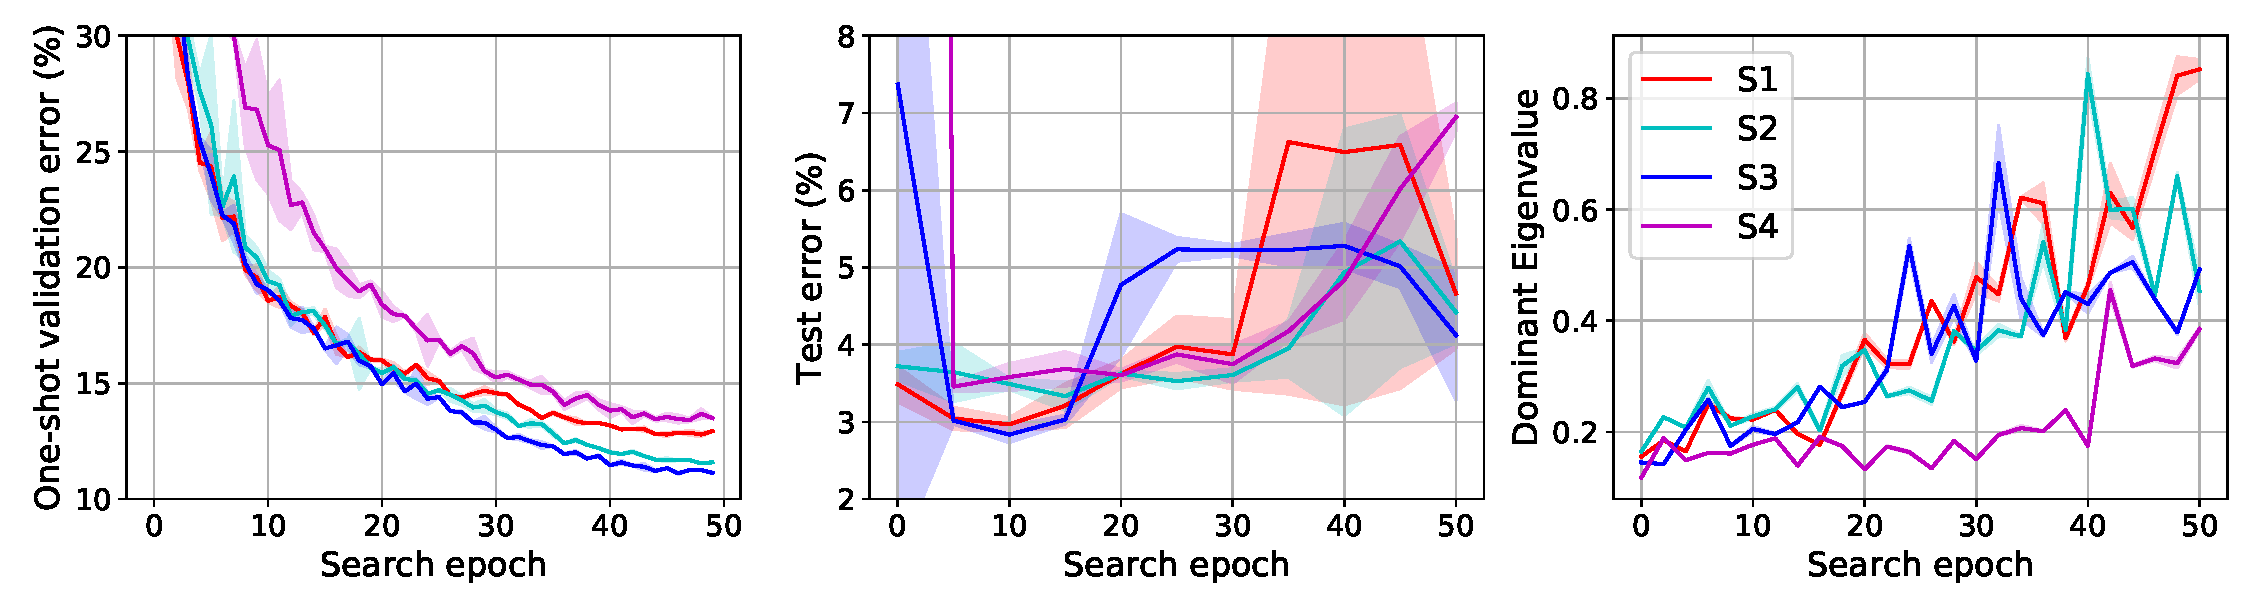
\includegraphics[scale=0.28]{images/valid_eigenvalues_traj.pdf}
}

}
%%%%%%%%%%%%%%%%%%%%%%%%%%%%%%%%%%%%%%%%%%%%%%%%%%%%%%%%%%%%%%%%%%%%%%%%%%%%%

%----------------------------------------------------------------------
\myframe{Questions to Answer for Yourself / Discuss with Friends}{

	\myit{
		\item Repetition:\\ \alert{What is the main difference between DARTS and with the previous one-shot NAS methods we saw?}
\bigskip
		\item Repetition:\\ \alert{How does DARTS optimize the architectural weights and one-shot weights?}
\medskip
		\item Discussion:\\ \alert{RobustDARTS early stops to a better architecture before the curvature of the validation loss becomes high. What is the intuition behind that? \textbf{HINT: think about the discretization step after the DARTS search.}}
	}	 
}
%-----------------------------------------------------------------------
